\section{Components for 3D Unstructured Mesh-based Workflows}

Automated, parallel, adaptive, simulation workflows require the
interactions of multiple software components.
Fig.~\ref{fig:workflowInteractions} shows the set of components needed for
reliable unstructured mesh simulations with a focus on the role of the parallel
mesh infrastructure.
To effectively support the integration with multiple parallel analysis
components, as well as alternative meshing and visualization technologies, the
parallel mesh structures and services interact through
APIs~\cite{BeaWal,Ollivier10}.
These APIs are designed specifically for an in-memory passing
of information that is needed between different simulation components in going
from the problem specification to the simulation results.
At the highest level, simulation information is specified in terms of attributes
on a description of the computational domain, typically a CAD model, and parameters
defining the physics model.
Boundary-based geometric model and mesh representations, building on the
abstraction of topological entities and their adjacencies, are ideally suited
for the specification of, and maintaining of, the relationship between domain
descriptions~\cite{beall1997general,garimella2002mesh,haimes2003unified}.
Problem definition attributes are transformed into mathematical fields
specified over geometric sub-domains, through the relationships between the
geometric model and mesh, while physics model parameters are transformed for
selection of partial differential equations and discretization methods.
Combined, this information is used to determine the desired output fields.
In the case of a mesh-based simulation, the domain information is discretized
into a mesh that is adapted during the simulation.
The mesh-based analysis discretizes the mathematical model and solves the
resulting algebraic systems to determine vectors of unknowns that correspond to
distribution coefficients for solution fields discretized over the mesh.

\begin{figure} \centering
  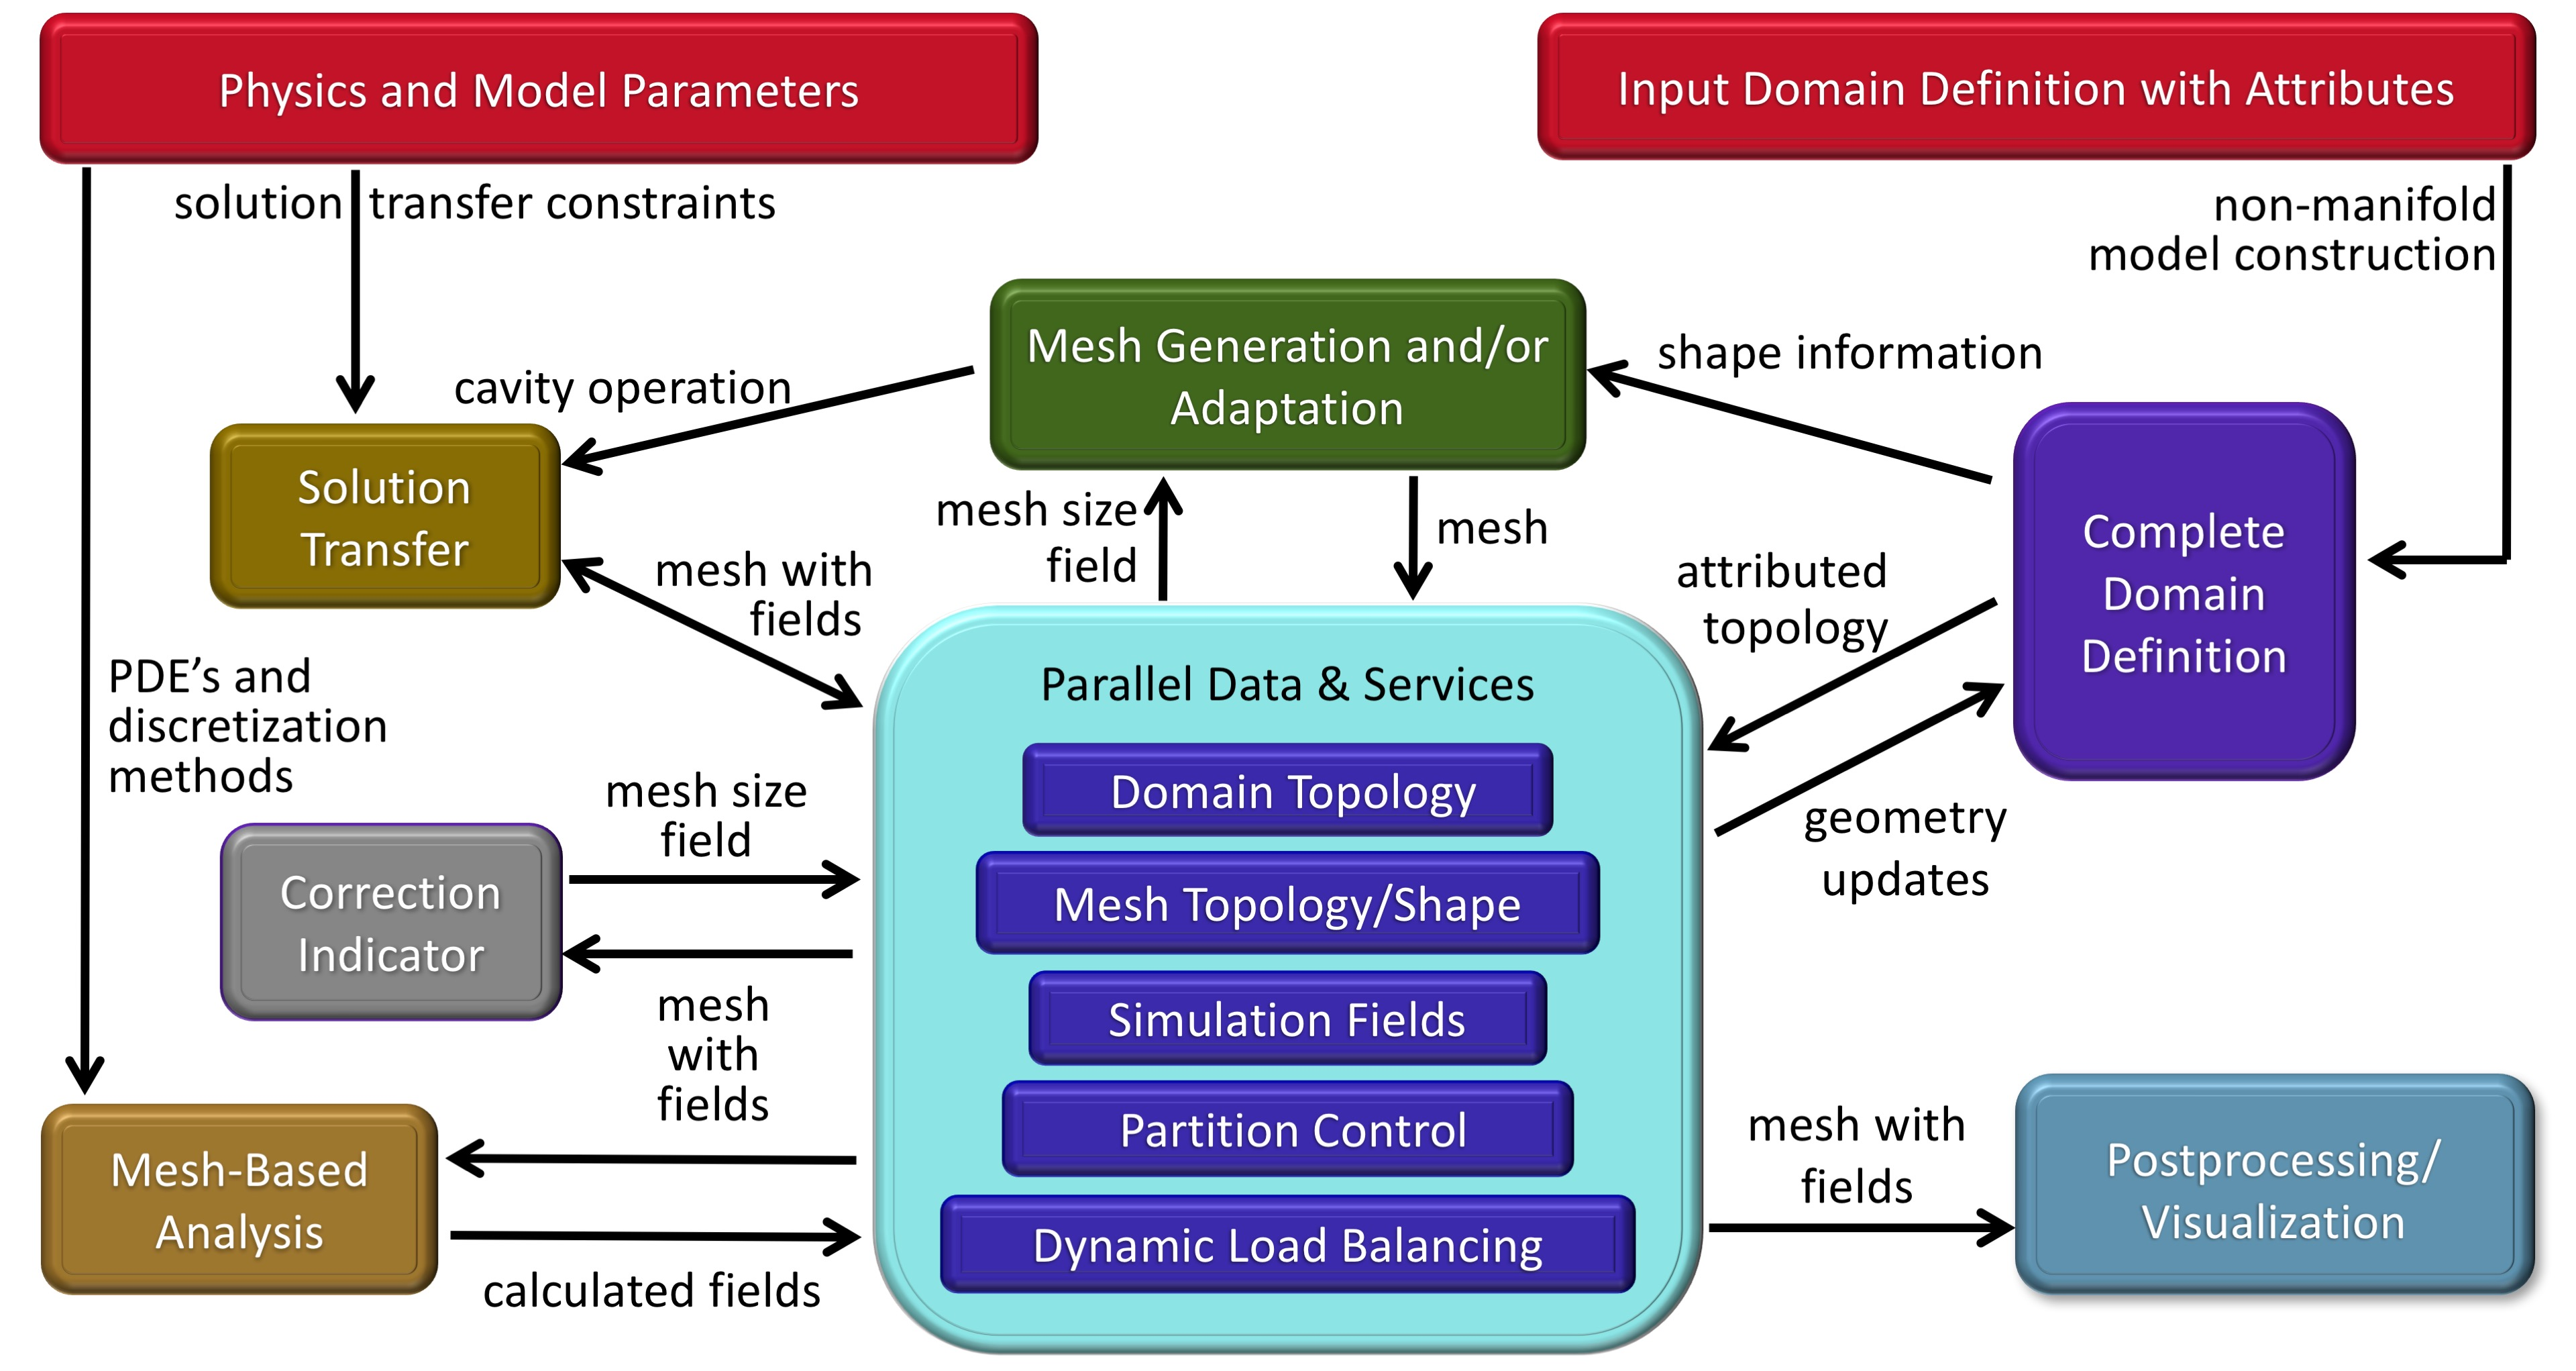
\includegraphics[width=.80\textwidth]{figures/workflowComponentInteractions.jpg}
  \caption{
    Components for parallel, adaptive, mesh-based simulation
    workflows~\cite{ibanez2016pumi}.
  }\label{fig:workflowInteractions}
\end{figure}

In the following sub-sections we review the functionality of the core
unstructured mesh workflow components depicted in
Fig.~\ref{fig:workflowInteractions} and available implementations.
A review of available partitioning tools is located in
Section~\ref{sec:partitioning}.

\subsection{Geometric Model Definition and Interrogation}

Non-manifold boundary representations provide an effective representation of the
computational domain that can be coupled with mesh generation/adaptation and
analysis attributes for the simulation workflow~\cite{BeaWal}.
Attribute information specified on topological entities of the geometric model
need to subsequently be related to the mesh discretizing the domain.
This critical association of a mesh entity to exactly one geometric model entity
of equal or higher order is known as classification.
Fig.~\ref{fig:geomclassification} depicts a two-dimensional geometric model
with four vertices, $G^0_{1-4}$, four edges, $G^1_{1-4}$, and one face, $G^2_1$,
and a mesh classified against it~\cite{ibanez2016pumi}.
The mesh faces are classified on the single geometric model face;
noted as $M^2_i \sqsubset G^2_1$.
Mesh edges $M^1_i$ adjacent to a single mesh face are classified on the
appropriate geometric model edges $G^1_{1-4}$.
All other mesh edges are classified on the geometric model face; a higher order
classification.
The mesh vertices at the corners of Fig.~\ref{fig:geomclassification} are
respectively classified against the geometric model vertices $G^0_{1-4}$.
Likewise, mesh vertices along the model edges $G^1_{1-4}$ are classified on
those edges.
The remaining unclassified interior mesh vertices are classified on the
geometric model face.

\begin{figure} \centering
  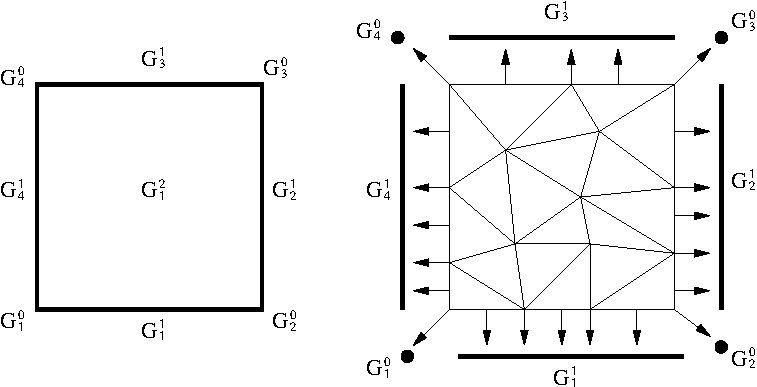
\includegraphics[width=.7\textwidth]{figures/gclas.pdf}
  \caption[A simple geometric model and a mesh classified on it.]{
    (left) A simple geometric model and (right) a mesh classified on
    it~\cite{ibanez2016pumi}.
    Arrows show the classification of boundary mesh vertices and edges to geometric model
    entities.
    The interior mesh vertices, edges, and faces are classified on the geometric
    model face $G^2_1$.}
  \label{fig:geomclassification}
\end{figure}

Some mesh data structures and geometric modeling interfaces also support a reverse
classification query.
Given a geometric model entity, this query will return the set of mesh entities
of equal order classified on it.
If provided, this query can improve the efficiency of transferring attribute
information associated with geometric model entities to mesh entities; the most
common example being boundary conditions.

In addition to topological information supporting classification, geometric
modeling interfaces can also provide geometric shape information to answer
positional queries and/or provide geometric shape parameters.
These queries enable operations of mesh adaptation and analysis components to
properly account for curved domains.
In mesh adaptation these queries are critical for positioning existing or new
vertices (or control points for higher order elements~\cite{DeyShephard_97})
such that the mesh can accurately tessellate the volume of the computational
domain.
Fig.~\ref{fig:edgesplit} depicts an example where a new mesh vertex is
positioned on the geometric model edge via a parametric location
query~\cite{beallthesis} or closest point projection.

\begin{figure} \centering
  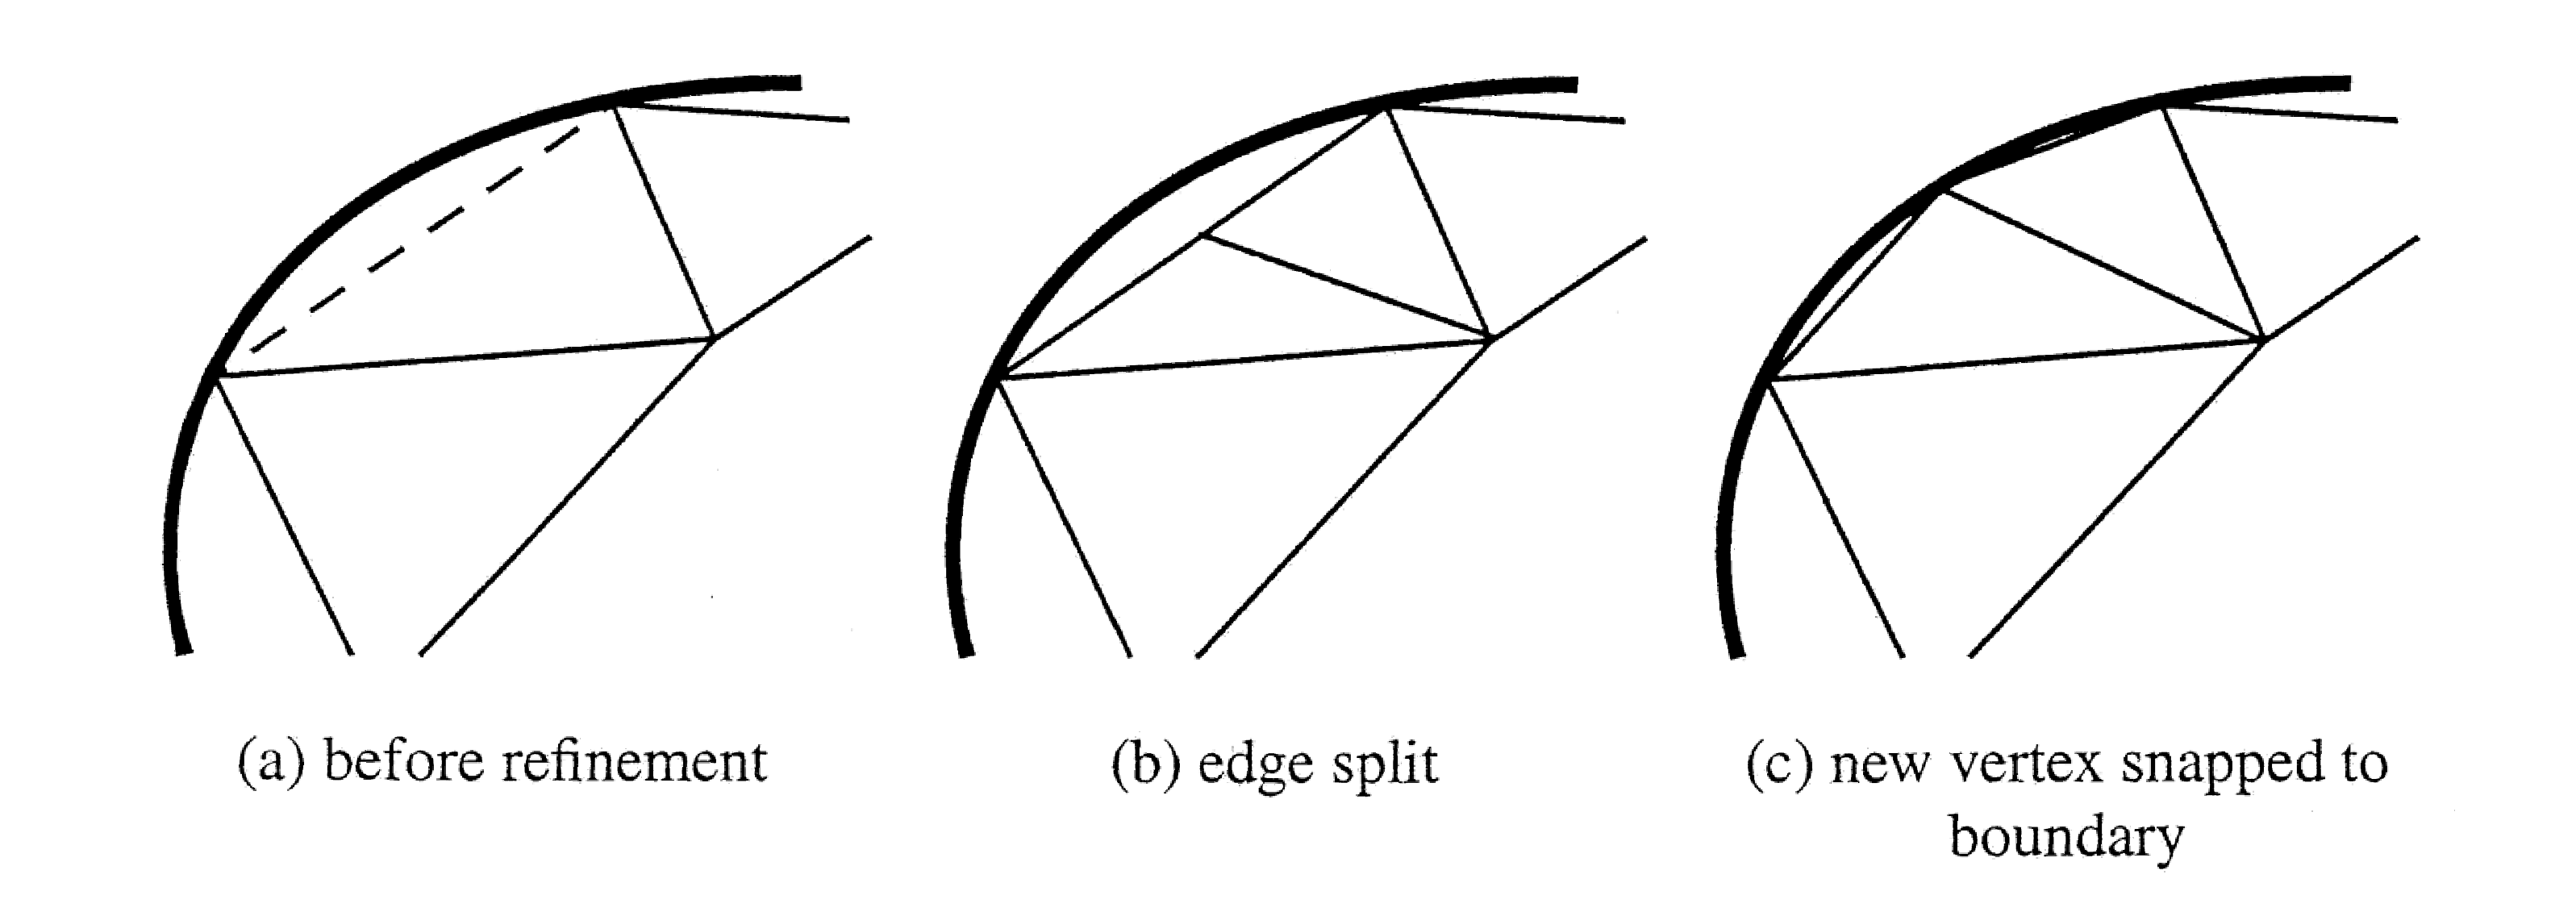
\includegraphics[width=.7\textwidth]{figures/edgesplit.eps}
  \caption{Mesh adaptation's use of a positional geometric model query to place a
    new mesh vertex on a geometric model edge~\cite{beallthesis}.}
  \label{fig:edgesplit}
\end{figure}

Outside of simulation workflows where engineers use CAD systems to design
devices are workflows where the computational domain information is provided in
a discrete form.
The most common forms of discrete domain information are triangulated surfaces,
voxel level forms, such as image data, and point clouds.
The source of this data can range from volumetric medical imaging (CT, PET,
etc.) of living tissues, to surface point clouds generated by satellite or LIDAR
imaging of geographical features.
Tools are available to convert this data to a topological representation of the
computational domain which can provide the fundamental classification queries
required by simulation workflows~\cite{klaasVoxel2014}.
However, there is limited functionality to recreate geometry information for
precisely satisfying positional queries on curved domain boundaries.
To fill this gap, surface reconstruction techniques are
available~\cite{carrRBFpointCloud2001,rusuPointCloud2011}.
Examples of voxel- and point cloud-based geometric model generation are
depicted in Fig.~\ref{fig:mouse} and Fig.~\ref{fig:landers}.
The resulting Digimouse~\cite{digiMouse2007} model supported adaptive mesh optimization for a
mesh-based Monte Carlo simulation of light propagation through tissues with
heterogeneous material
properties~\cite{meshMonteCarlo2014,edmansMeshMonteCarlo2015}.
The latter example of the Landers fault system supported petascale high order
dynamic rupture earthquake simulations that were an SC '14 Gordon Bell
Finalist~\cite{seisSolGordonBell2014}.

\begin{figure} \centering
  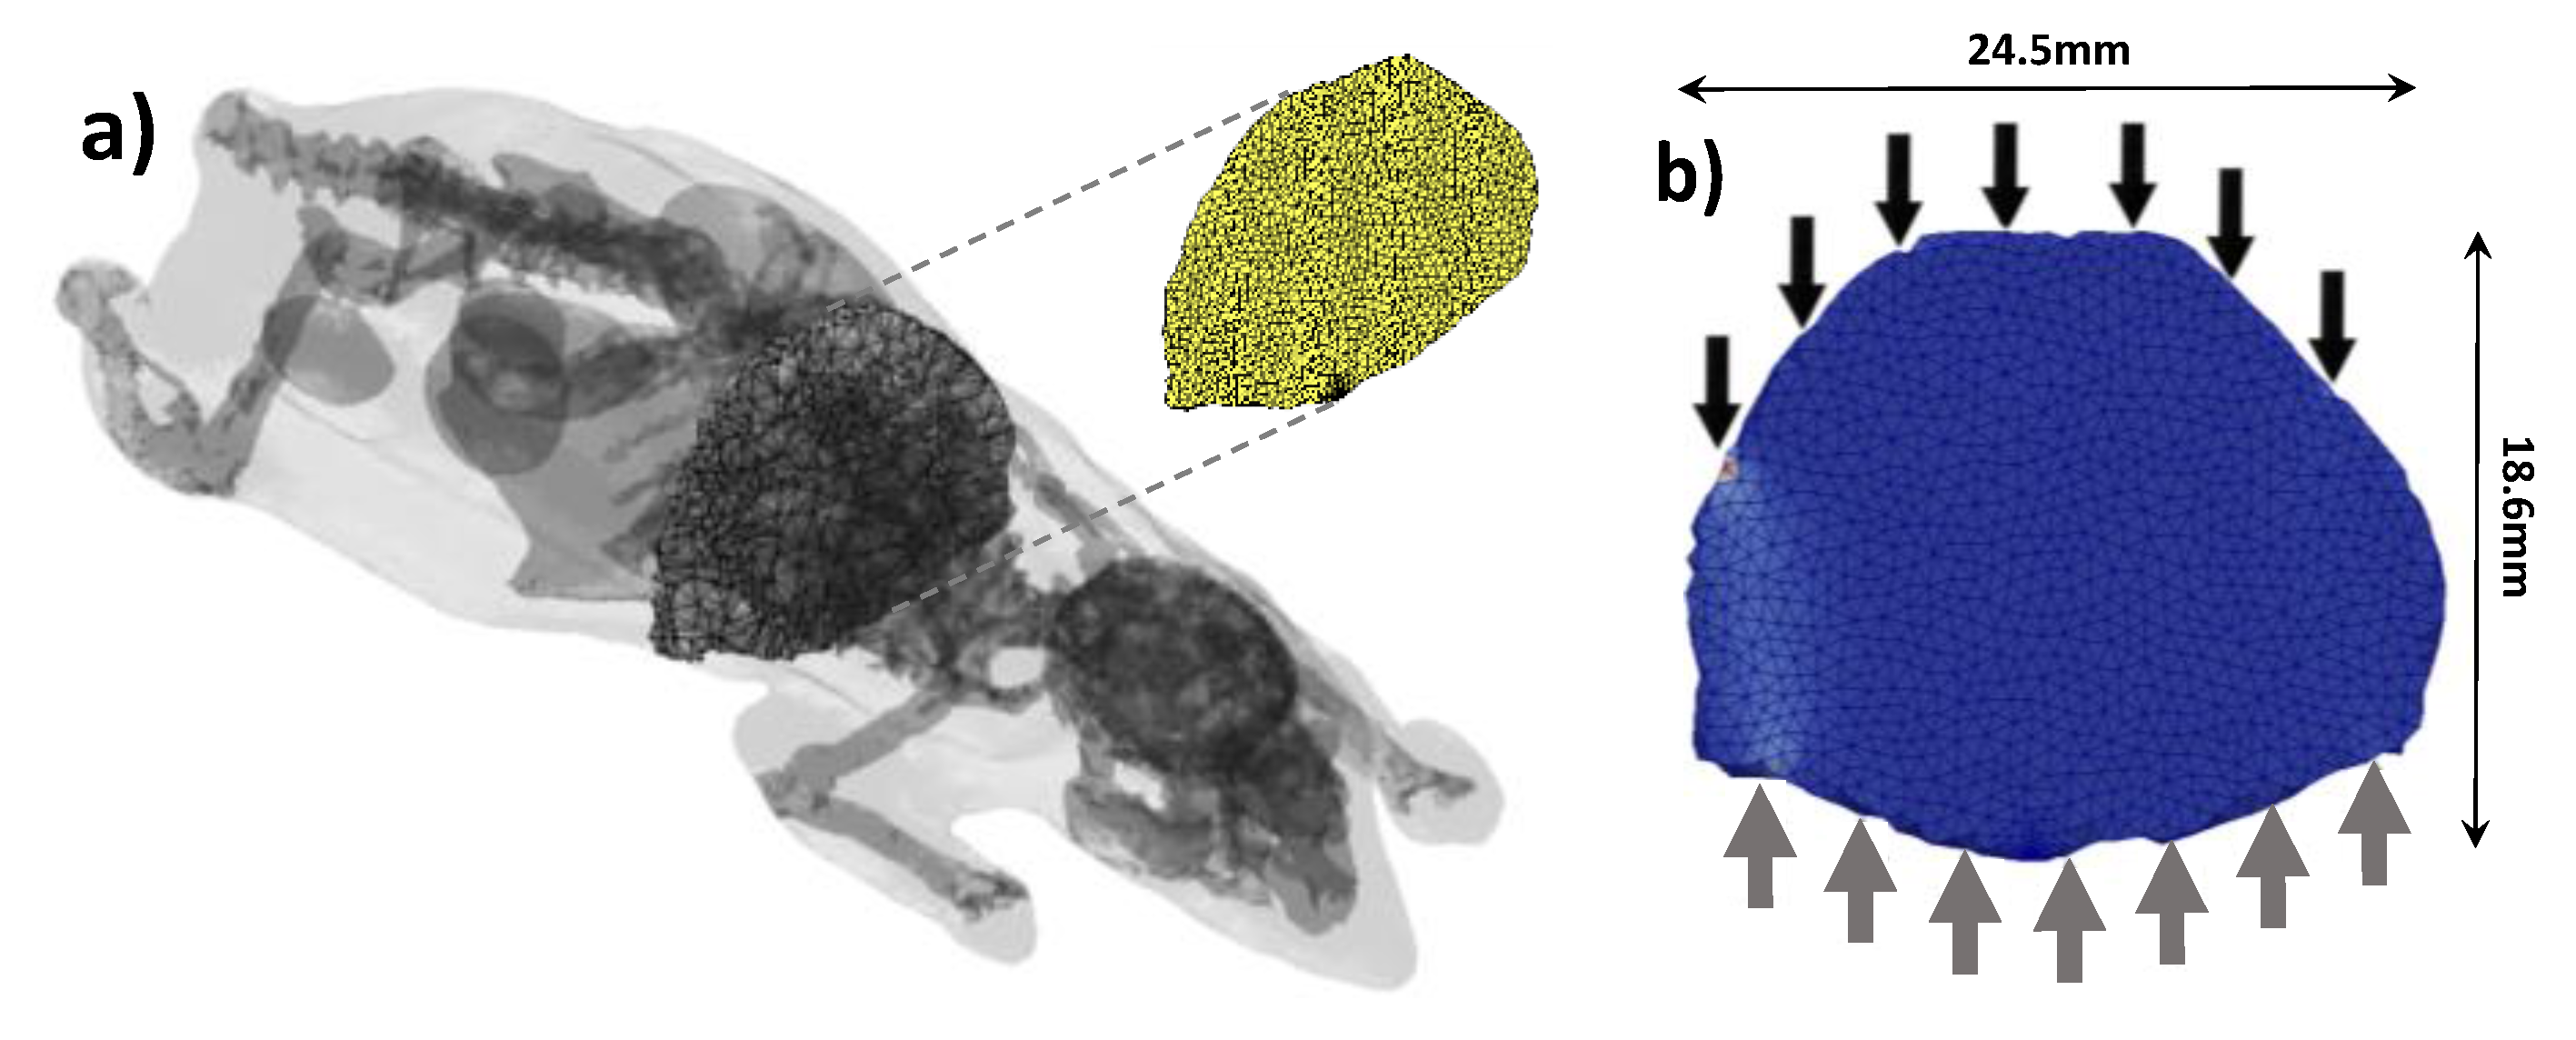
\includegraphics[width=.8\textwidth]{figures/digimouse_edmans.png}
  \caption{The mesh of a 2D slice through the segmented Digimouse created using
    Simmetrix GeomSim.
    The location of light emitters and detectors are shown with black and gray
    arrows, respectively~\cite{edmansMeshMonteCarlo2015}.}
  \label{fig:mouse}
\end{figure}

\begin{figure} \centering
  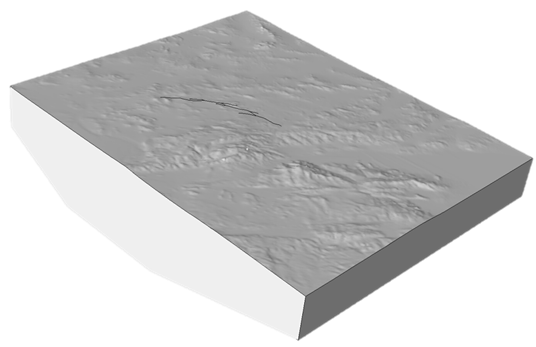
\includegraphics[width=.3\textwidth]{figures/landersMdl.png}
  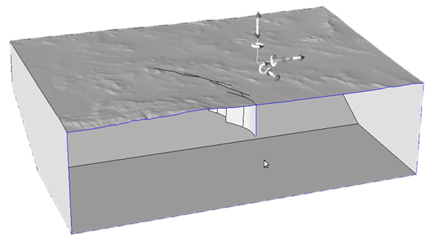
\includegraphics[width=.3\textwidth]{figures/landersMdl_cut.png}
  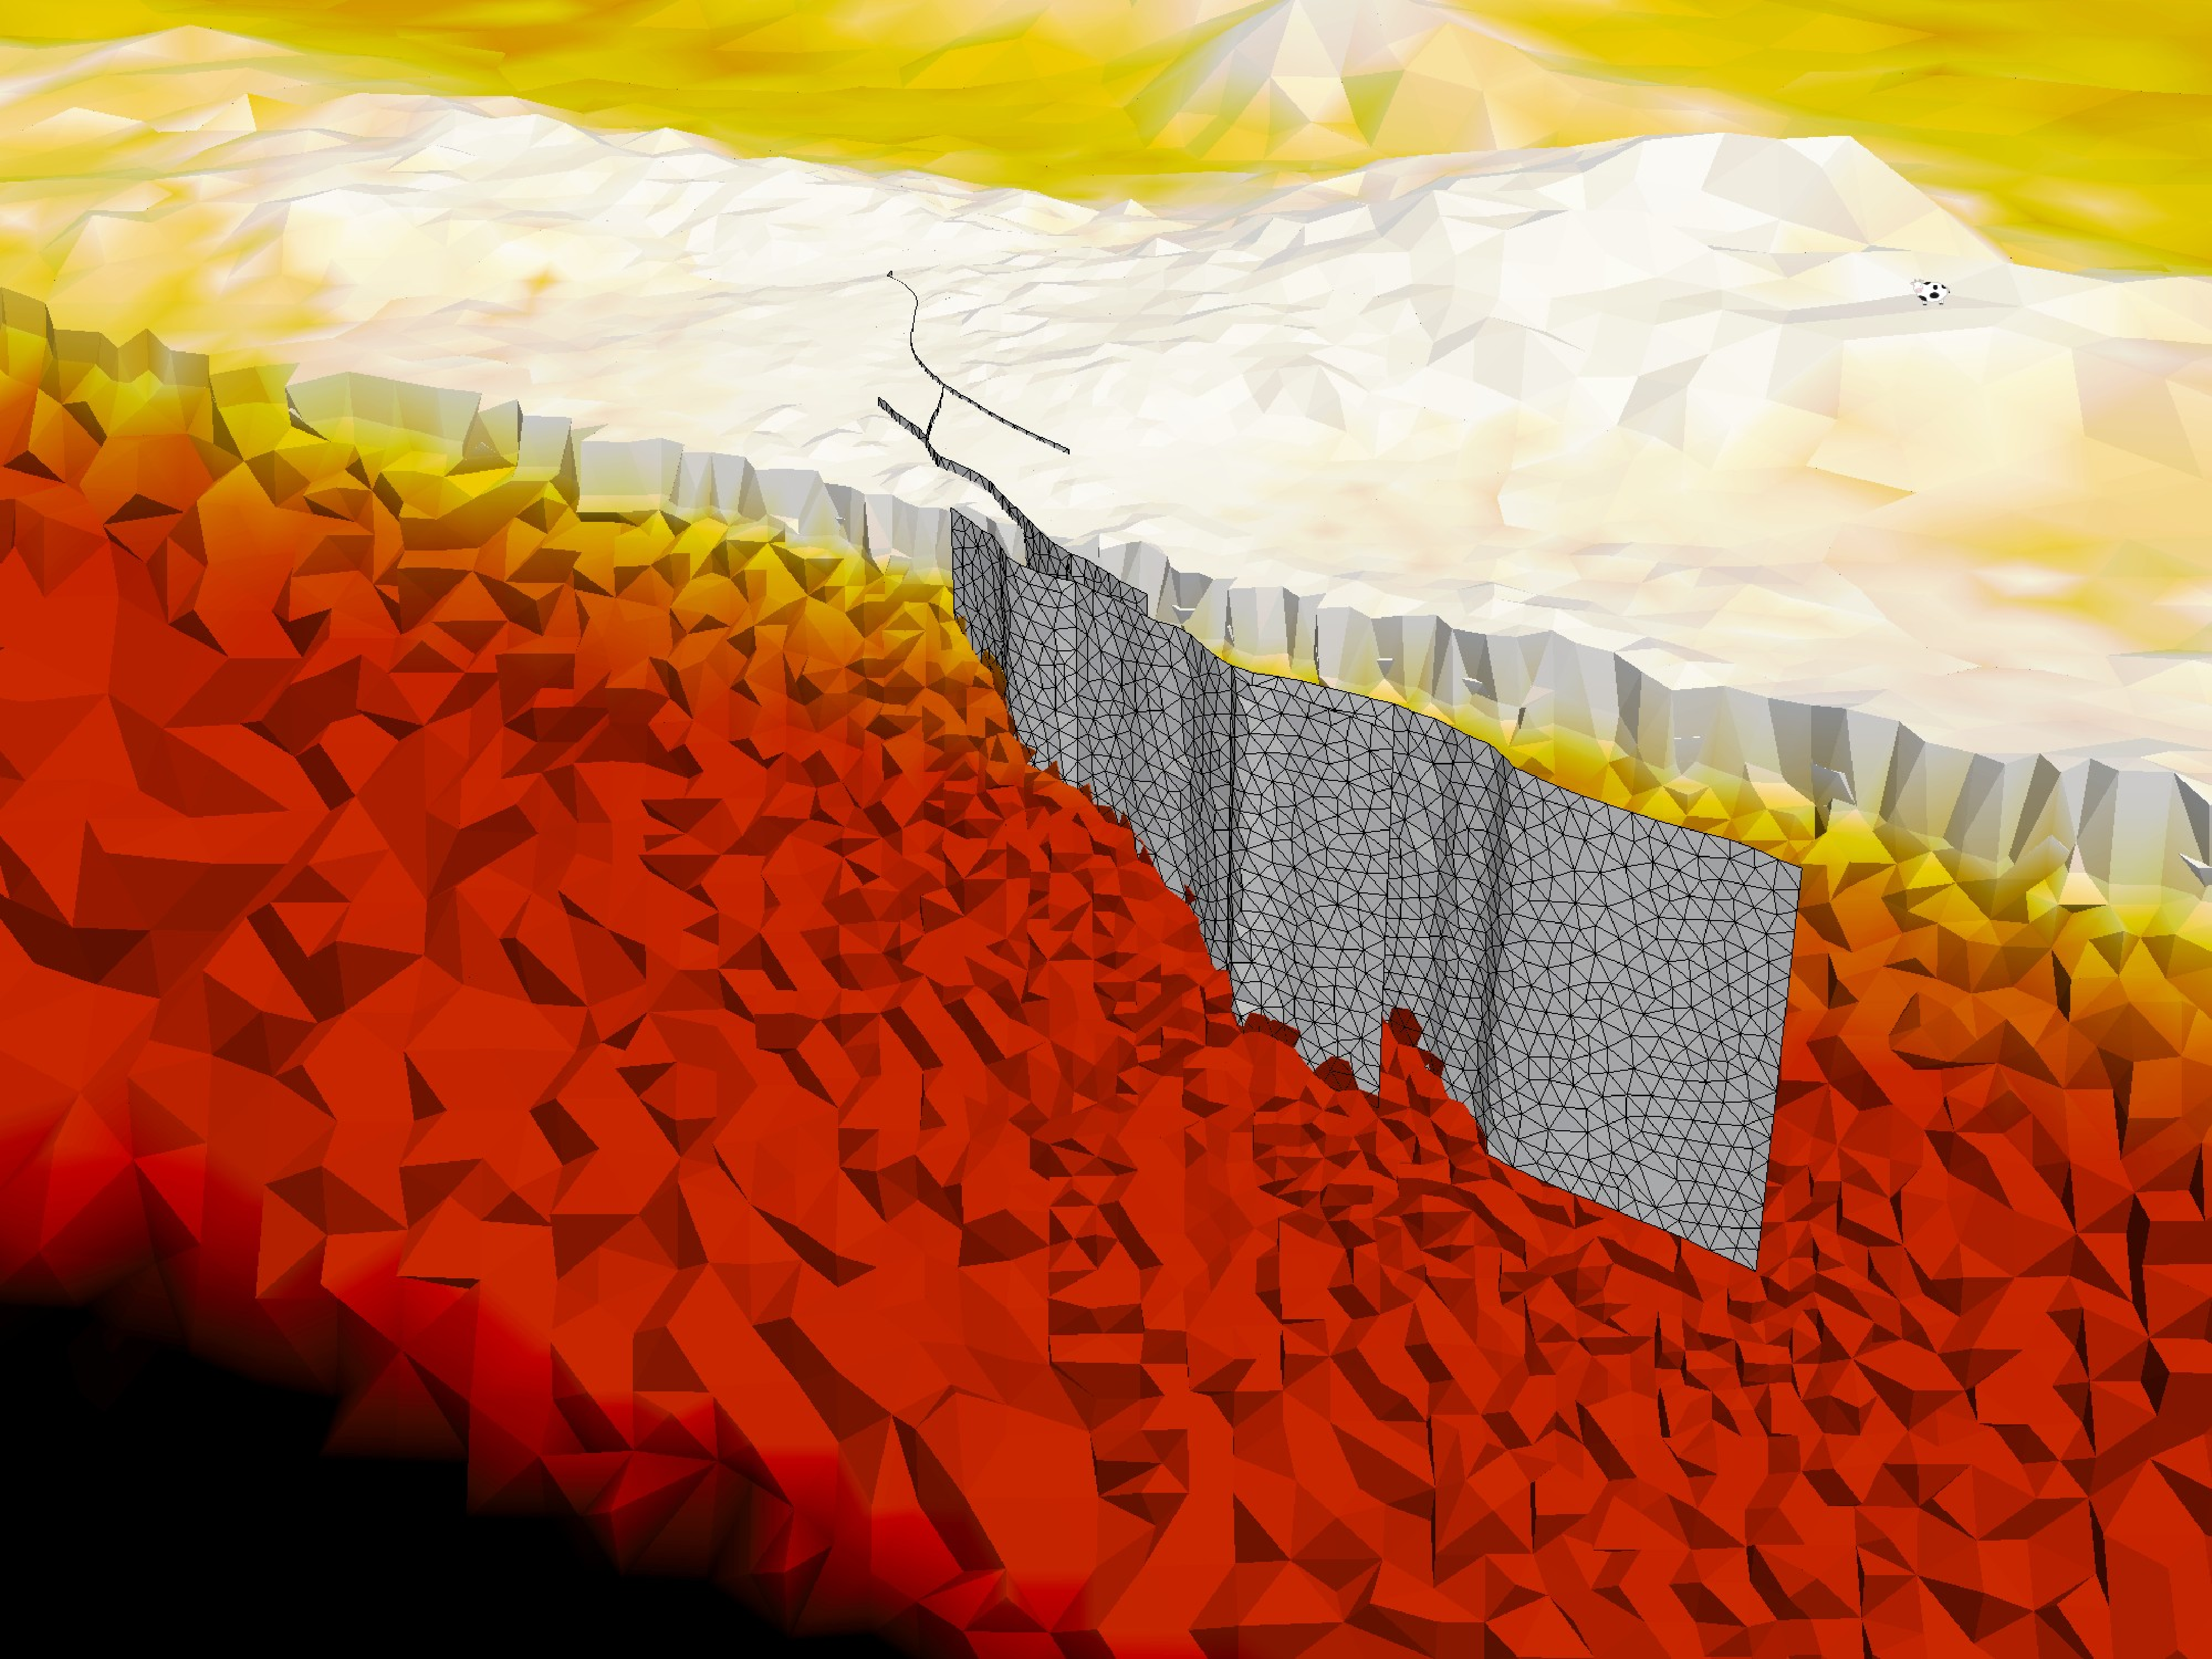
\includegraphics[width=.6\textwidth]{figures/landersMesh.pdf}
  \caption{(top) Geometric model and (bottom) mesh of the Landers
    fault system for SeisSol dynamic rupture earthquake
    simulations~\cite{seisSolGeomPoster,seisSolGordonBell2014}.}
  \label{fig:landers}
\end{figure}

A robust, closed-source component that supports workflow interactions with both
discrete and parametric geometric models is
GeomSim~\cite{simmodsuite} from Simmetrix.
Its functionality is provided through functional interfaces to several CAD
systems (NX, Pro/E, SpaceClaim, and SolidWorks) and modeling kernels (Parasolid,
ACIS, and Granite).
Built on those interfaces, it has capabilities to correct poorly defined
geometry, perform boolean operations on multiple CAD models (both discrete and
parametric), automatically remove small features, when desired, and create
complementary domains.

Applications which require an entirely open-source workflow can use components
built upon the open-source (LGPL) Open CASCADE~\cite{opencascade_web} modeling
kernel.
Unfortunately, its usability is hampered by a lack of documentation and a code
base with over two million lines.
To address the usability issues, the Common Geometry
Module~\cite{sigma_web,cgm_bitbucket,tautges2001cgm} (BSD-3 derivative) and
EGADS~\cite{haimesEgads2012} (LGPL) systems provide a simplified
interface over Open CASCADE.
Along with OpenCSM, a library for specifying sequences of geometric
construction operations provided by EGADS, the Engineering
Sketch Pad provides a web-enabled system for construction of parametric
geometry used for automated design optimization~\cite{haimesEngSketchPad2013}.

\subsection{Mesh Generation}

To avoid the mesh generation bottleneck in simulation workflows a mesh generator
must be (1) fully automated, (2) include methods for creating desired mesh types
and gradations (including anisotropic meshes), and (3) be driven from a geometric
model-based specification of the mesh control information.
Given a valid, properly toleranced geometric model, an automated mesh generator
is one that executes to completion without user interaction; including the case
where no size controls are set~\cite{autoMeshGen1992}.
By definition, there can be no requirement for the user to operate on individual
mesh entities to `repair' the mesh.
Such a robust mesh generator must rely on geometric model kernels for accurate
answers to topological and positional queries.

The Simmetrix MeshSim and distributed memory Parallel MeshSim
components satisfy the mesh generation requirements.
Parallel MeshSim can generate a one billion element mesh on a CAD model
in about six minutes on 224 Intel Xeon processors.
Meshes with up to 13 billion elements have been generated on 2048 processors.
In this thesis the majority of the meshes generated were done so with the
Simmetrix tools.

Another closed-source mesh generator that meets the requirements is from
Pointwise~\cite{pointwise_web,pointwise_aiaa_2007}.
Unlike, MeshSim though, they only support shared memory parallelism.
Thus, the size of the initial mesh they generate is limited by the amount of
memory available on the system.
There are also several serial open-source mesh generators that partially meet the
requirements:
gmsh (GPL)~\cite{geuzaine2009gmsh},
NETGEN (LGPL)~\cite{netgen_Schoberl1997},
and GRUMMP (BSD derivative)~\cite{grummp2011,freitag1997tetrahedral}.

\subsection{Mesh Adaptation}

As transient simulations evolve, the areas of the computational domain with large
discretization error will also change.
Procedures to automatically change the spatial discretization, the mesh, to
control these errors are required.
To operate effectively mesh adaptation procedures must run in parallel, apply
local modification operations towards satisfaction of the applications requests,
conform to the definition of the computational domain, and provide application
`hooks' to support the transfer of fields and other data associated with the
mesh as it is modified.

Applications specify how they need the mesh to change through a
three-dimensional metric tensor at each mesh
vertex~\cite{loseille2015parallel,compere2010mesh,li20053d}.
The tensor defines how edges incident to each vertex should be rotated and
scaled to reduce the discretization error.
For example, in the proximity of a shock the gradients normal to the front will be
much higher than those along the front.
As such, an application can define the tensor using derivatives of the quantity
of interest to capture this anisotropy.
In many applications though, it is sufficient to define isotropic scaling.
For these cases the size field can be expressed as a scalar at each mesh
vertex.

PUMI's parallel mesh adaptation component (MeshAdapt) meets
the requirements by supporting refinement, coarsening, and nodal
repositioning~\cite{ibanez2016pumi}.
With each local mesh modification operation applied (split, collapse, swap, etc.)
fields on the mesh are transferred.
Field transfers are supported through interpolation and projection operations in
the topological proximity of the modified mesh
entities~\cite{ibanezthesis}.
For fields with higher continuity or conservation requirements
Omega\_h~\cite{osh_github,ibanez2016mesh} (BSD-2-Clause) provides
the necessary transfer mechanisms along with the majority of the PUMI MeshAdapt
functionality~\cite{ibanez2016mesh,ibanezthesis}.

The Simmetrix SimModSuite Parallel MeshSimAdapt~\cite{simmodsuite}
satisfies the requirements while also providing more advanced support for meshes
with stacks of semi-structured elements (e.g., often found in meshes used
for solving flow problems with boundary layers).
MeshSimAdapt procedures have executed on meshes as large as 92 billion
elements on 786,432 cores~\cite{rasquinCise2014}.

Like MeshAdapt and MeshSimAdapt, the LGPL licensed
MAdLib implements advanced mesh motion and local mesh modification
operators, but only on tetrahedral meshes in serial~\cite{compere2010mesh}.
Another serial open-source adaptation code is GRUMMP.
It provides mesh quality improvement via edge/face swaps, and vertex
re-positioning, but coarsening procedures are focused on supporting multi-grid
methods.

%From the TOMS paper
%many unstructured mesh data structures have been introduced
%to date such as AHF [Dyedov et al 2014], libMesh [Kirk et al. 2006], MOAB
%[Tautges
%2004], OpenVolumeMesh [Kremer et al. 2013], etc. H

\subsection{Mesh Data Structures}

Components that answer questions about mesh topology and permit association of
field data are referred to as mesh data structures.
A distributed memory parallel mesh data structure must also support the queries
to determine the links between entities that are classified on part
boundaries.
Parallel data structures typically also support some level of ghosting; the
copying of one or more layers of mesh entities across the part boundaries
for read-only access~\cite{misbahGhosting2013}.

Mesh data structures that support mesh adaptation must also support topological
modifications and the migration of mesh entities between processes.
Such modifiable mesh data structures are far more complex as efficient storage
becomes a challenge.
For example, a mesh entity of a given order (vertex, edge, face, region) has a
fixed number of downward adjacencies depending on its topological type
(triangle, quadrilateral, tetrahedron, prism, hexahedron, etc.).
But, the upward adjacencies are only bounded by the quality the mesh; meshes
with poor quality tend to have high-degree vertices (characterized by their
one-to-many vertex-to-edge fan out).

Currently, the most memory efficient parallel mesh data structures that support
adaptation are those using structures-of-arrays (SoA)~\cite{ibanez2016pumi}.
While SoA implementations are not as intuitive as their object-based brethren,
the complexity can be hidden under an object-based interface that significantly
increases ease of use.
A more recent benefit of SoA implementations is their data-parallel
friendliness.
On devices such as GPUs with thousands of small compute units, or CPUs with wide
vector units, memory accesses are most efficient when they can be combined
together into a fewer larger transfers
(coalescing)~\cite{nickolls2008scalable,karlRuppStridedAccess}.
Since SoA implementations allocate large contiguous arrays where each entry
represents a mesh entity or some scalar data associated with an entity, then an
algorithm that traverses the mesh (dependency/collision issues aside) will
implicitly have unit-stride coalesced accesses.
That is in stark contrast to the irregular memory access pattern when
traversing an object-based implementation where each object is individually
allocated (to reduce the dynamic resizing complexities).
An array-of-structs (AoS) implementation could avoid the irregular access
pattern by pre-allocating the structs, but still suffer from non unit-stride
access penalties~\cite{karlRuppStridedAccess}.
As mesh data structure algorithms are memory bandwidth bound, the
run time advantage of SoA implementations over object-based can be significant.

APF\_MDS~\cite{ibanez2016pumi} (BSD-3-Clause) and
Omega\_h both provide parallel
modifiable mesh data structures implemented using SoA.
APF\_MDS provides distributed memory parallelism via MPI and
supports PUMI's MeshAdapt implementation.
Omega\_h supports hybrid super computers through MPI for
inter-process communications and Kokkos~\cite{edwards2013kokkos} for
intra-process shared memory communication and computation.
MOAB (LGPL) is an alternative array-based distributed memory parallel
mesh data structure that supports
modification~\cite{tautges2004moab}.


